\section{Results}
\label{sec:results}

\subsection{The latent interface is substantially less accurate than retaining text}

Table~\ref{tab:accuracy} reports both scoring rules for every primary condition.
Across the three main bridge seeds, synthetic test accuracy is
$4.3\%\pm2.0$ percentage points (mean $\pm$ sample standard deviation),
compared with 53.1\% for PLaMo translation followed by ordinary target input.
The main bridge mean is 1.0\% on the wording holdout and 1.6\% on MGSM.
All three main seeds score 4/250 on MGSM; equal aggregate scores do not establish
stability beyond these three fits.
Layer and prefix changes leave bridge test accuracy between 2.0\% and 4.3\%
at seed 11.
None approaches the textual alternatives in this experiment.

\begin{table}[htbp]
\caption{Primary evaluation accuracy: strict / last-number exact match (\%)}
\label{tab:accuracy}
\centering\small\sffamily
\begin{tabular}{@{}lrrr@{}}
\toprule
Condition & Test ($n=256$) & Wording holdout ($n=128$) & MGSM ($n=250$) \\
\midrule
Frozen text: Japanese & 10.5 / 39.5 & 11.7 / 43.0 & 1.2 / 9.2 \\
Frozen text: paired English & 17.6 / 50.8 & 21.9 / 57.0 & --- \\
Frozen text: PLaMo translation & 14.8 / 53.1 & 18.8 / 54.7 & 0.8 / 25.6 \\
Bridge $L8,K16$, seed 11 & 4.3 / 4.3 & 1.6 / 1.6 & 1.6 / 1.6 \\
Bridge $L8,K16$, seed 23 & 6.2 / 6.2 & 0.8 / 0.8 & 1.6 / 1.6 \\
Bridge $L8,K16$, seed 37 & 2.3 / 2.3 & 0.8 / 0.8 & 1.6 / 1.6 \\
Bridge $L4,K16$, seed 11 & 2.7 / 2.7 & 2.3 / 2.3 & 1.2 / 1.2 \\
Bridge $L16,K16$, seed 11 & 3.1 / 3.1 & 0.8 / 0.8 & 1.6 / 1.6 \\
Bridge $L8,K4$, seed 11 & 2.0 / 2.0 & 2.3 / 2.3 & 1.2 / 1.2 \\
Untrained bridge $L8,K16$ & 1.6 / 2.0 & 1.6 / 2.3 & 0.8 / 1.6 \\
Shuffled bridge $L8,K16$ & 0.4 / 0.4 & 1.6 / 1.6 & 1.2 / 1.2 \\
Learned textual prefix $K16$ & 73.8 / 73.8 & 60.2 / 60.2 & 8.0 / 8.0 \\
\bottomrule
\end{tabular}
\par\smallskip\footnotesize
$L$ is the source layer and $K$ the prefix length. The untrained and shuffled
controls use seed 11, as does the learned textual prefix. The latter retains
Japanese question text and receives the same task supervision as the bridge;
the three frozen text systems receive no such fitting. Paired English templates
are available only for the generated tasks. Values are rounded for display;
raw counts and predictions remain in the result files.
\end{table}

The learned textual prefix reaches 189/256 (73.8\%) on the synthetic test and
77/128 (60.2\%) on the wording holdout, with 24,576 trainable parameters.
It is more accurate here than the 2,360,832-parameter bridge despite having fewer
trainable parameters.
On MGSM it reaches 20/250 (8.0\%), so the controlled-task improvement does not
establish a general natural-language reasoning benefit.
Figure~\ref{fig:accuracy} displays the conditions with per-condition uncertainty.

\begin{figure}[htbp]
\centering
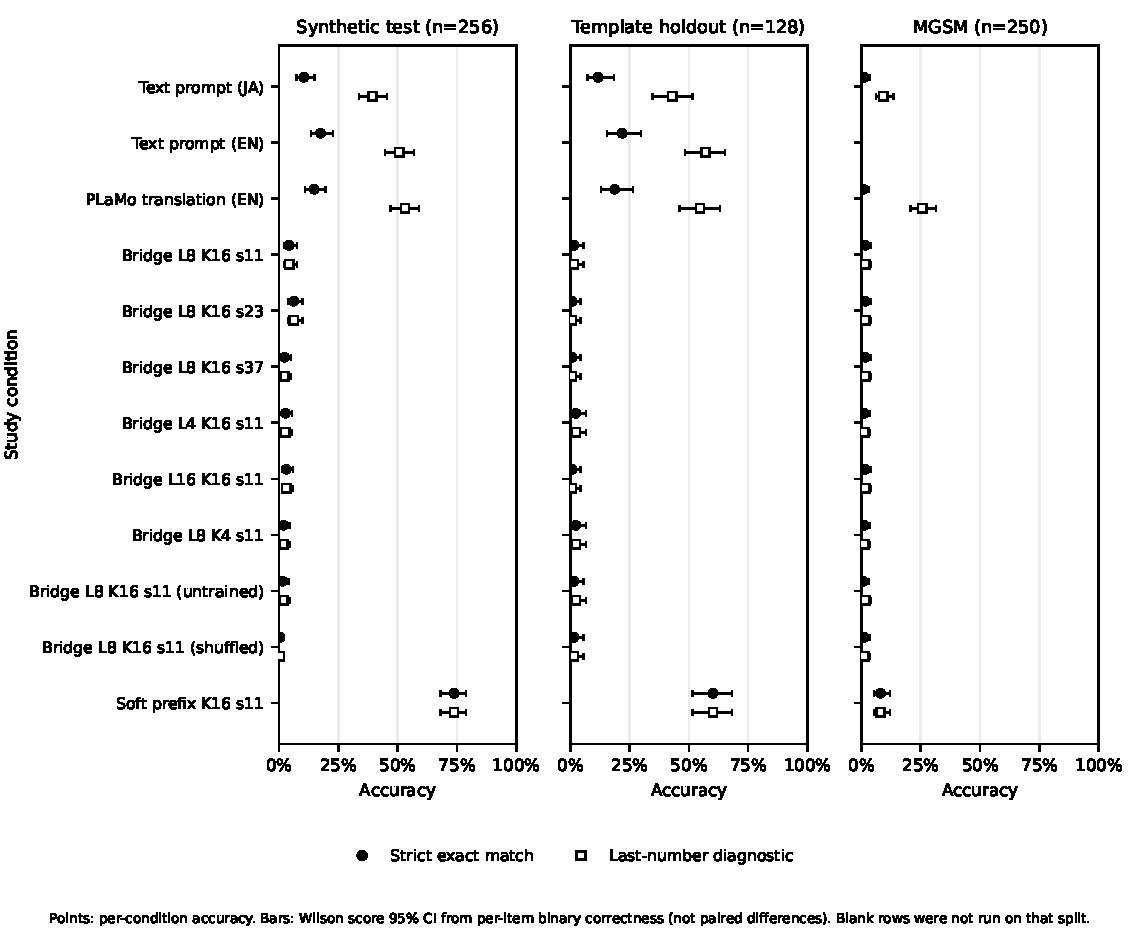
\includegraphics[width=\linewidth]{accuracy_comparison.pdf}
\caption{Primary condition accuracies. The panels show synthetic test questions,
the separate wording holdout and Japanese MGSM. Marker shapes distinguish strict
exact match from the last-number diagnostic. Intervals are 95\% Wilson score
intervals for per-item binary correctness, conditional on each fitted model.
They describe individual proportions; paired effect intervals are reported
separately in Table~\ref{tab:contrasts}. The paired English MGSM condition is
unavailable, rather than zero.}
\label{fig:accuracy}
\end{figure}

\subsection{Output format materially changes the apparent ranking}

On MGSM, the main bridge's strict score of 1.6\% exceeds the frozen translation
pipeline's 0.8\%, whereas the last-number diagnostic reverses the comparison to
1.6\% versus 25.6\%.
The strict score alone would therefore give a misleading impression of answer
quality.
The latent systems almost always emit short numeric answers, consistent with
their answer-only training target.
The frozen systems often emit explanations despite the numeric-only instruction.

No PLaMo translation reaches its translation cap: all 256 test, 128 wording-holdout
and 250 MGSM translations terminate normally.
Answer generation has a different pattern.
The frozen PLaMo-translation pipeline reaches the answer cap on 38/256 synthetic
test questions, 26/128 wording-holdout questions and 119/250 MGSM questions.
The direct Japanese system reaches it on 1/256, 1/128 and 30/250, respectively.
The trained bridges and learned textual prefix have no answer-cap hits on these
three endpoints.
These results compare finite-budget pipelines; longer explanations and the
last-number rule both limit their interpretation as underlying reasoning ability.

\subsection{Source correspondence matters on the synthetic test, but the effect is small}

For the main seed-11 bridge, shuffling source prefixes reduces synthetic test
accuracy from 11/256 to 1/256.
The paired difference is 3.9 percentage points, with a 95\% bootstrap interval of
$[1.6,6.6]$ points (Table~\ref{tab:contrasts}).
This is evidence that the fitted interface uses source correspondence for some
correct answers in this test set.
The last-number contrast against the untrained bridge is less decisive:
2.3 points with interval $[-0.4,5.1]$.
On the wording holdout and MGSM, the shuffled contrasts include zero.
The result therefore supports limited input dependence rather than broad
transfer of reasoning ability.

\begin{table}[htbp]
\caption{Selected paired contrasts in last-number exact match (percentage points)}
\label{tab:contrasts}
\centering\small\sffamily
\begin{tabular}{@{}llrr@{}}
\toprule
Endpoint & Contrast & Difference & 95\% paired interval \\
\midrule
Synthetic test & Bridge $-$ shuffled & $+3.9$ & $[1.6,6.6]$ \\
Synthetic test & Bridge $-$ untrained & $+2.3$ & $[-0.4,5.1]$ \\
Synthetic test & Translation $-$ bridge & $+48.8$ & $[42.2,55.5]$ \\
Synthetic test & Bridge $-$ textual prefix & $-69.5$ & $[-75.4,-63.3]$ \\
Wording holdout & Bridge $-$ shuffled & $0.0$ & $[-3.1,3.1]$ \\
MGSM & Bridge $-$ shuffled & $+0.4$ & $[-1.6,2.4]$ \\
MGSM & Translation $-$ bridge & $+24.0$ & $[18.4,29.6]$ \\
MGSM & Bridge $-$ textual prefix & $-6.4$ & $[-10.0,-3.2]$ \\
\bottomrule
\end{tabular}
\par\smallskip\footnotesize
Bridge contrasts use the preselected main $L8,K16$, seed-11 fit.
Translation denotes actual PLaMo translation followed by frozen target text input.
Intervals use 10,000 paired item resamples; contrast signs follow the displayed
subtraction. These are exploratory, conditional intervals without correction for
multiple comparisons, rather than equivalence tests.
\end{table}

\subsection{The textual prefix improves single-step arithmetic, not all task families}

Table~\ref{tab:operations} shows that the learned textual prefix's high synthetic
overall score comes from single-step questions.
It answers 183/192 of those items correctly, but only 6/64 two-step items.
The paired-English and PLaMo-translation systems perform better on the two-step
family under the last-number diagnostic.
The learned textual prefix thus does more than change output format on the
single-step tasks, while its success remains strongly task dependent.

\begin{table}[htbp]
\caption{Synthetic test last-number accuracy by task family (\%, $n=64$ per cell)}
\label{tab:operations}
\centering\small\sffamily
\begin{tabular}{@{}lrrrr@{}}
\toprule
Condition & Addition & Subtraction & Multiplication & Two-step \\
\midrule
Frozen Japanese text & 59.4 & 42.2 & 43.8 & 12.5 \\
Frozen paired-English text & 65.6 & 45.3 & 56.2 & 35.9 \\
Frozen PLaMo translation & 71.9 & 51.6 & 57.8 & 31.2 \\
Main bridge, seed 11 & 3.1 & 6.2 & 1.6 & 6.2 \\
Shuffled main bridge & 1.6 & 0.0 & 0.0 & 0.0 \\
Learned textual prefix & 96.9 & 93.8 & 95.3 & 9.4 \\
\bottomrule
\end{tabular}
\end{table}

Figure~\ref{fig:learning} shows decreasing training and validation losses for the
three main bridge fits.
Their selected validation losses are 1.205, 1.197 and 1.258, respectively.
The learned textual prefix instead selects epoch 9 with validation loss 0.349.
The main seed-11 bridge also achieves only 89/1,024 (8.7\%) when freely generating
answers for its own training questions after fitting.
The failure therefore cannot be attributed solely to unseen test questions:
the main training run itself has low answer accuracy at the selected budget.

\begin{figure}[htbp]
\centering
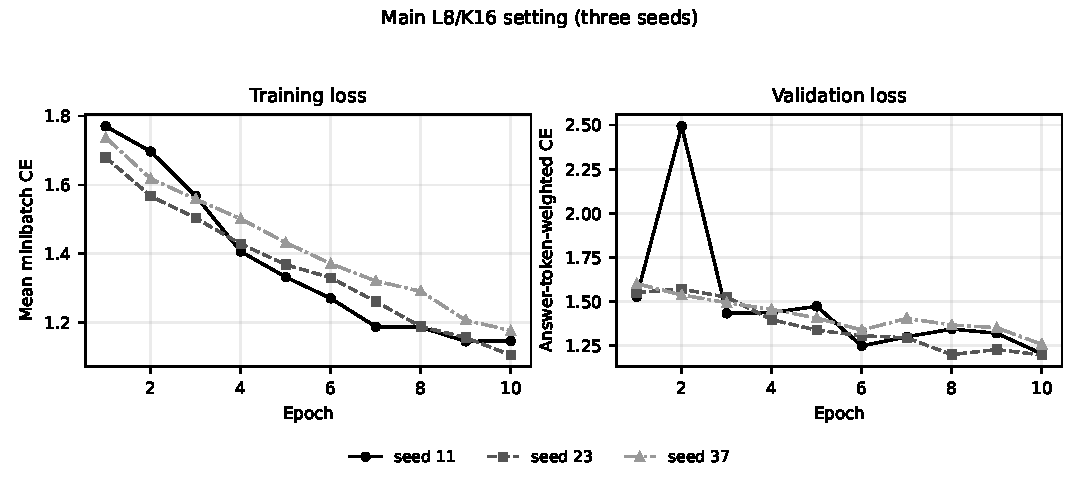
\includegraphics[width=\linewidth]{learning_curves.pdf}
\caption{Main $L8,K16$ bridge learning curves for seeds 11, 23 and 37.
Training curves average minibatch answer-token cross-entropies; validation
curves weight loss by the number of supervised answer tokens.
All pretrained backbone parameters remain fixed.
Checkpoint selection uses validation loss, while the primary task scores come
from independent free-running generation rather than teacher forcing.}
\label{fig:learning}
\end{figure}

\subsection{Post hoc capacity check: a small mapping can be memorized}

The low primary scores motivated a separate capacity diagnostic after the main
matrix had completed.
A newly initialized main-architecture bridge was fitted to 16 generated questions
with data seed 20261110, batch size 8 and 100 epochs.
For this diagnostic only, validation was an exact copy of those training items,
and checkpoint selection minimized resubstitution loss.
The dataset metadata explicitly marks the intended overlap.
This condition measures memorization capacity, not held-out performance, and
changes both dataset size and the number of exposures per question.

The fitted bridge answers all 16 training questions correctly.
When their source prefixes are shuffled, only 3/16 answers match the original
target references, but all 16 outputs equal the answer associated with the
\emph{supplied source} question.
The three remaining target matches consist of one fixed point in the permutation
and two coincident reference answers.
Thus the interface can memorize a small source-dependent mapping; its poor main
result is not evidence that the computational path is incapable of transmitting
any learned correspondence.
Together with the main fit's 8.7\% training accuracy, the diagnostic points to
difficulty fitting the larger problem under the selected representation and
optimization budget, rather than a failure confined to unseen questions.
It does not identify which architectural or training change would resolve that
difficulty.

The diagnostic has its own configuration, data, histories, source-shuffle mapping
and raw predictions under \path{overfit_diagnostic}; its resubstitution scores are
excluded from Table~\ref{tab:accuracy} and the primary accuracy figure.

